\documentclass[a4paper, 12pt, oneside]{report}

\usepackage[english, italian]{babel}
\usepackage[utf8]{inputenc}
\usepackage[autostyle=true]{csquotes}
\usepackage{graphicx}
\usepackage[backend=biber, backref=true]{biblatex}
\addbibresource{ref.bib}
\setlength{\parskip}{1em}
\usepackage{geometry}
\usepackage{setspace}
\usepackage{hyperref}

% Opzioni stile capitoli
\usepackage[Rejne]{fncychap}
\makeatletter
\renewcommand*{\@makechapterhead}[1]{%
  \vspace*{5\p@}%
  {\parindent \z@ \raggedright \normalfont
    \ifnum \c@secnumdepth >\m@ne
      \if@mainmatter%%%%% Fix for frontmatter, mainmatter, and backmatter 040920
        \DOCH
      \fi
    \fi
    \interlinepenalty\@M
    \if@mainmatter%%%%% Fix for frontmatter, mainmatter, and backmatter 060424
      \DOTI{#1}%
    \else%
      \DOTIS{#1}%
    \fi
  }}
% For the case \chapter*:
\renewcommand*{\@makeschapterhead}[1]{%
  \vspace*{5\p@}%
  {\parindent \z@ \raggedright
    \normalfont
    \interlinepenalty\@M
    \DOTIS{#1}
    \vskip 5\p@
  }}
  \ChNameVar{\centering\large\rm}
\makeatother


\begin{document}
\newgeometry{margin=1in}
\begin{titlepage}
\noindent
  \begin{minipage}[t]{0.2\textwidth}
    \vspace{-4mm}{
\includegraphics[scale=1.2]{img/logo_unimib.pdf}}
  \end{minipage}
  \begin{minipage}[t]{0.78\textwidth}
    {
      {    
      \textsc{Università degli Studi di Milano - Bicocca}}
      \vspace{4.5mm} \\
      \setstretch{1.2}
      \textbf{Scuola di Scienze} \\
      \textbf{Dipartimento di Informatica, Sistemistica e Comunicazione} \\
      \textbf{Corso di laurea in Informatica}
      
    }
  \end{minipage}
  
  \vspace{40mm}
  
  \begin{center}
    {\LARGE{
        \setstretch{1.3}
        \textbf{Una soluzione mobile based a supporto della terapia cognitivo comportamentale}}}
  \end{center}
  
  \vspace{40mm}

  \noindent
  {\large \textbf{Relatore:} \textit{Chiari.ma Prof.ssa Daniela Micucci} }
  
  \noindent
  {\large \textbf{Correlatore:} \textit{Chiari.mo Dott. Davide Ginelli}}
  
  \vspace{15mm}

  \begin{flushright}
  
    \textbf{\large Relazione della prova finale di:} \\
    \large{\textit{Ionut Daniel Fagadau}}\\
    \large{\textit{Matricola 845279}}
  \end{flushright}
  
  \vspace{40mm}
  \begin{center}
    {\large{\bf Anno Accademico 2020-2021}}
  \end{center}
  
\end{titlepage}
%\newpage\null\thispagestyle{empty}\newpage
\restoregeometry

\tableofcontents

\cleardoublepage
\phantomsection
\addcontentsline{toc}{chapter}{Introduzione}
\chapter*{Introduzione}

\textbf{Depressione} e \textbf{ansia} sono i problemi più comuni sperimentati dagli studenti universitari; questo è dovuto al fatto che quello universitario è un periodo decisivo della vita di ogni persona che si
ritrova a dover prendere molte decisioni importanti per il proprio futuro e a doversi adattare ad ambienti nuovi, spesso anche a città nuove.
Tutti questi fattori possono portare a grandi quantità di \textbf{stress} che può determinare la nascita di problematiche maggiori.

È ormai risaputo che questo genere di disturbi è spesso più diffuso tra gli studenti universitari \textit{(circa il 30\% degli studenti universitari soffre di depressione)} \cite{MilanoSFU} e spesso tutto questo sfocia in problematiche ancora più gravi (istinti suicidi, abuso di sostanze, autolesionismo, ...).
È chiaro dunque che esiste un problema legato alla salute mentale degli studenti che va
affrontato il prima possibile per evitare ripercussioni più gravi; molte istituzioni spesso mettono a disposizione del personale con cui trattare questi argomenti ma, purtroppo, non tutti sono disposti a parlare dal vivo dei propri problemi, che sia per vergogna o per mancanza di disponibilità. Non solo, in un periodo come questo appena vissuto, in cui una pandemia ha colpito il mondo intero, è ancor più difficile per chi soffre di questo tipo di problemi potersi mettere in contatto con chi di dovere.

Per questo motivo è utile e necessario avere una via alternativa, che possa essere percorsa anche da chi non ha disponibilità agli incontri dal vivo, all'identificazione e potenziale trattamento di questo genere di patologie. L'idea è utilizzare la tecnologia che usiamo già giorno per giorno per svolgere innumerevoli altri compiti.
Lo scopo di questo progetto è dunque la realizzazione di un'applicazione a supporto della salute mentale che permetta, tramite degli \textbf{\textit{screening}}, di identificare potenziali patologie accusate da uno studente e di affrontare un percorso di guarigione costituito da \textbf{video-lezioni} ed \textbf{esercizi}, composti da questionari in diversa forma, mirati ad aumentare la consapevolezza del paziente sulle sue patologie e su come trattarle giorno per giorno.
Le lezioni e gli esercizi saranno erogati settimanalmente, proprio come se fossero delle vere sedute dallo psicologo, in modo da permettere un trattamento graduale e il tutto sarà gestito in maniera anonima proprio per permettere la partecipazione anche a chi non è disposto a parlare apertamente.
L'applicazione inoltre si occuperà di mantenere attivo il rapporto con l'utente tramite dei semplici questionari quotidiani che verranno notificati ad un orario a scelta arbitraria.

L'applicazione è stata sviluppata utilizzando il framework di Google \textbf{Flutter}, che utilizza il linguaggio di programmazione \textbf{Dart}. La scelta di utilizzare questa tecnologia è supportata dal fatto che Flutter permette di avere un'unica code base da cui poter compilare applicazioni sia per \textbf{iOS} che per \textbf{Android}, i due sistemi operativi leader nel mercato degli smartphone.
Non solo, con la recente pubblicazione di Flutter 2, è possibile utilizzare la stessa code base per compilare anche applicazioni \textbf{web} stabili e applicazioni per Google \textbf{Fuchsia}, il nuovo sistema operativo di Google. Possiamo quindi affermare con sicurezza che la scelta di utilizzare Flutter mira, oltre che alla semplicità di sviluppo per diverse piattaforme, al supporto di tecnologie future.

Nel capitolo \textit{MindBlooming} sono spiegati in dettaglio gli obiettivi dell'applicazione e le funzionalità che essa offre, mentre il capitolo \textit{Progettazione} entra nel dettaglio di come sono effettivamente gestite queste funzionalità e con quali strumenti. Nel capitolo \textit{Implementazione} invece sono descritti i componenti utilizzati per costruire l'applicazione, come sono stati costruiti e come sono stati risolti i problemi incontrati durante lo sviluppo. Infine, nel capitolo \textit{Manuale Utente} è presente una guida all'utilizzo dell'applicazione dal punto di vista degli utenti.
\chapter{MindBlooming}
\section{Interventi Internet Based}

Diversi studi hanno dimostrato come degli interventi internet-based, ovvero virtuali, aiutassero i pazienti che soffrono di disturbi psichici\cite{taylor2003computer}; in particolare alcuni studi riguardavano l'utilizzo di messaggi di testo sotto forma di promemoria, messaggi di supporto e/o procedure di auto-monitoraggio come terapia, con risultati positivi.
In un mondo in cui la tecnologia è sempre più presente nelle nostre vite, ad esempio grazie agli \textbf{smartphone} la cui crescita in continuo aumento è osservabile nella Figura \ref{fig:smartphone_users}, questi studi rappresentano un'opportunità per permettere sempre a più persone di disporre di una terapia che altrimenti potrebbero rigettare \textit{(per mantenere l'anonimato, per questioni di tempo o per qualsiasi altro motivo)}.

\section{Dispositivi Mobile}
Secondo l'articolo in costante aggiornamento di \textbf{bankmycell}\cite{bankmycell}, sono circa 3.8 miliardi le persone che utilizzano uno smartphone al giorno d'oggi con oltre 10 miliardi di connessioni mobile attive; si stima che per il 2023 gli utilizzatori di smartphone saliranno a 7.33 miliardi. Sempre nello stesso articolo viene mostrato come \textbf{Apple} abbia la più grossa fetta del mercato mobile col suo \textbf{iOS}, seguita dalle case produttrici di smartphone che implementano \textbf{Android} asserendo quindi il dominio di questi due sistemi operativi nel mondo mobile.

\begin{figure}
\centering
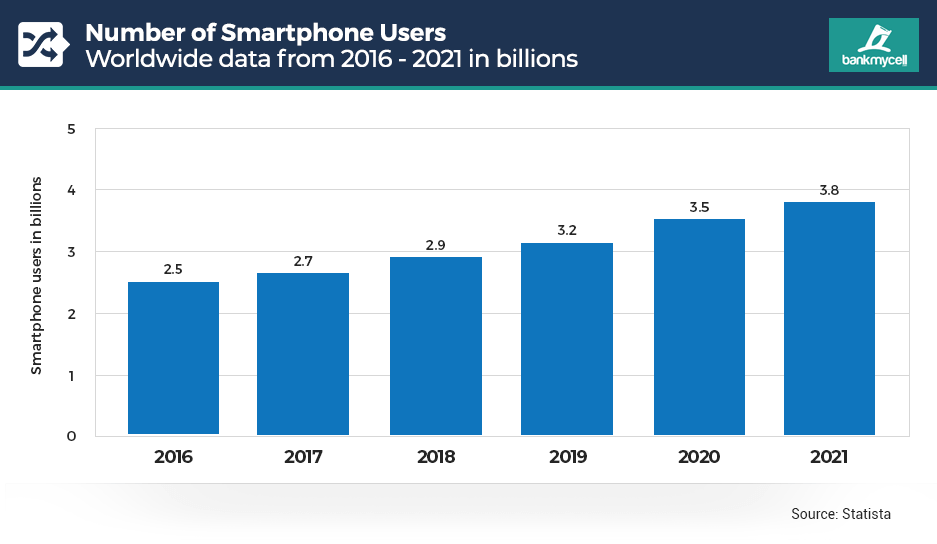
\includegraphics[width=\textwidth]{img/smartphone_users}
\caption{Numero di utilizzatori di smartphone nel mondo \cite{bankmycell}}
\label{fig:smartphone_users}
\end{figure}

\section{mHealth}
Lo sviluppo di questi studi e la diffusione degli smartphone nel mondo ha portato a quella che è chiamata \textbf{mHealth} \textit{(o mobile health)}; la messa in pratica della medicina e della salute pubblica supportata dall'utilizzo di dispositivi mobile\cite{mHealth}.
La mHealth è una parte di quella che viene chiamata \textbf{eHealth}, ovvero l'utilizzo di dispositivi informatici e tecnologici \textit{(dai computer ai monitor dei pazienti)} per il supporto dei servizi salutari.
Questo tipo di tecnologie permette oggi anche a paesi sottosviluppati di avere accesso ad una assistenza sanitaria di qualche tipo per permettere di identificare e curare in tempo eventuali disturbi.

Tra i vari servizi resi disponibili dalla mHealth ci sono anche quelli \textbf{educativi} del paziente sui disturbi di cui soffre, quelli di \textbf{helpline} che forniscono al paziente un contatto con esperti del settore e quelli di \textbf{remote disease surveillance} che permettono al paziente di diventare consapevole dei propri disturbi ed eventualmente sostenere un percorso di guarigione \textit{(che sia online o meno)}, che è esattamente quello a cui miriamo con la nostra applicazione.

\section{Strategie Principali}
Come abbiamo detto, il vantaggio principale delle pratiche come mHealth sono l'accesso in
maniera anonima e la libera scelta di un orario, fattori sicuramente positivi per il target d'udienza dell'applicazione, ovvero gli studenti universitari.
Per quanto riguarda l'identificazione e lo sviluppo di cura dei disturbi psichici, alcune strategie chiave sono il \textbf{monitoraggio dell'umore} del soggetto, la raccomandazione di \textbf{attività che scoraggino i pensieri negativi}, l'\textbf{educazione} del soggetto sui propri disturbi e l'\textbf{accesso alle reti di supporto} da parte di esso; tutte queste strategie fanno parte della \textbf{Terapia Cognitivo-Comportamentale} \cite{CBT} che è un metodo di cura adatto al trattamento individuale ed è finalizzata a trattare i pensieri negativi, le emozioni disfunzionali e i comportamenti disadattivi del paziente in modo da facilitare l'eliminazione dei disturbi psicologici.

\section{Funzionalità Offerte}
Dunque, scopo finale dello stage è stato quello di realizzare un'applicazione di mHealth che permetta agli utenti, nel nostro caso agli studenti universitari, di auto-educarsi sui disturbi di cui potrebbero soffrire tramite un'attività iniziale di \textbf{screening} atta ad identificare segnali d'allarme che possano suggerire la presenza di tali disturbi, e l'eventuale \textbf{educazione} e \textbf{mitigazione} di essi tramite attività di monitoraggio dell'umore, \textbf{lezioni didattiche} sui propri disturbi e su come combatterli, \textbf{esercizi attivi} per il recupero.
Questo sarà eseguito utilizzando dei questionari accompagnati da contenuti multimediali da
completare settimanalmente, uniti a una parte di domande giornaliere per il monitoraggio
dell'utente. I questionari sono creati sulla piattaforma \textbf{Qualtrics}, nata inizialmente per gestire dei questionari di tipo aziendale, che permette di definire diversi tipi di domande e di inserire vari media nelle domande stesse, offrendo l'accesso a tutto ciò tramite API.
Verrà inoltre tenuta traccia dei progressi dell'utente e, utilizzando un calendario, verranno segnalati nuovi esercizi ogni volta che questi sono disponibili. Per permettere un monitoraggio del soggetto sono inoltre disponibili delle domande giornaliere che verranno notificate all'utente ad un orario a sua scelta.


\chapter{Progettazione}
Prima di poter mettere mano all'applicazione è stato necessario un iniziale periodo di studio dell'ambiente, in particolare del linguaggio \textbf{Dart} e del framework \textbf{Flutter}; è stato piacevole scoprire come Flutter supporti nativamente sia il \textbf{Material Design}, stile adottato per lo sviluppo dell'interfaccia grafica \textit{(almeno per quanto riguarda Android)}, sia lo stile \textbf{Cupertino}, ovvero lo stile nativo di iOS, impostando di default alcune regole di tali stili quando vengono creati determinati widget.

Successivamente a questo periodo di studio è iniziata la vera e propria progettazione dell'applicazione, fase durante la quale sono stati stabiliti il modello dei dati e l'architettura adottata per lo sviluppo.

\section{Prima di Qualtrics}
Inizialmente non era stato scelto uno specifico backend, per cui lo sviluppo del modello dati è stato eseguito pensando ad un generale database e ad una generica applicazione che facesse uso di domande e risposte. Come possiamo osservare nella Figura \ref{fig:modello_iniziale}, è stato pensato ad un modello estremamente semplice ma estendibile e che, per il momento, distingueva solo domande a risposta aperta, domande a risposta chiusa e domande \textit{"speciali"} di screening (che inizialmente pensavamo fossero solo a risposta chiusa).
Ad ogni domanda erano poi associate delle opzioni selezionabili \textit{(o definibili nel caso di domande a risposta aperta)} e la risposta ad una certa domanda non era altro che l'opzione \textit{(o le opzioni)} selezionata.

\begin{figure}
\centering
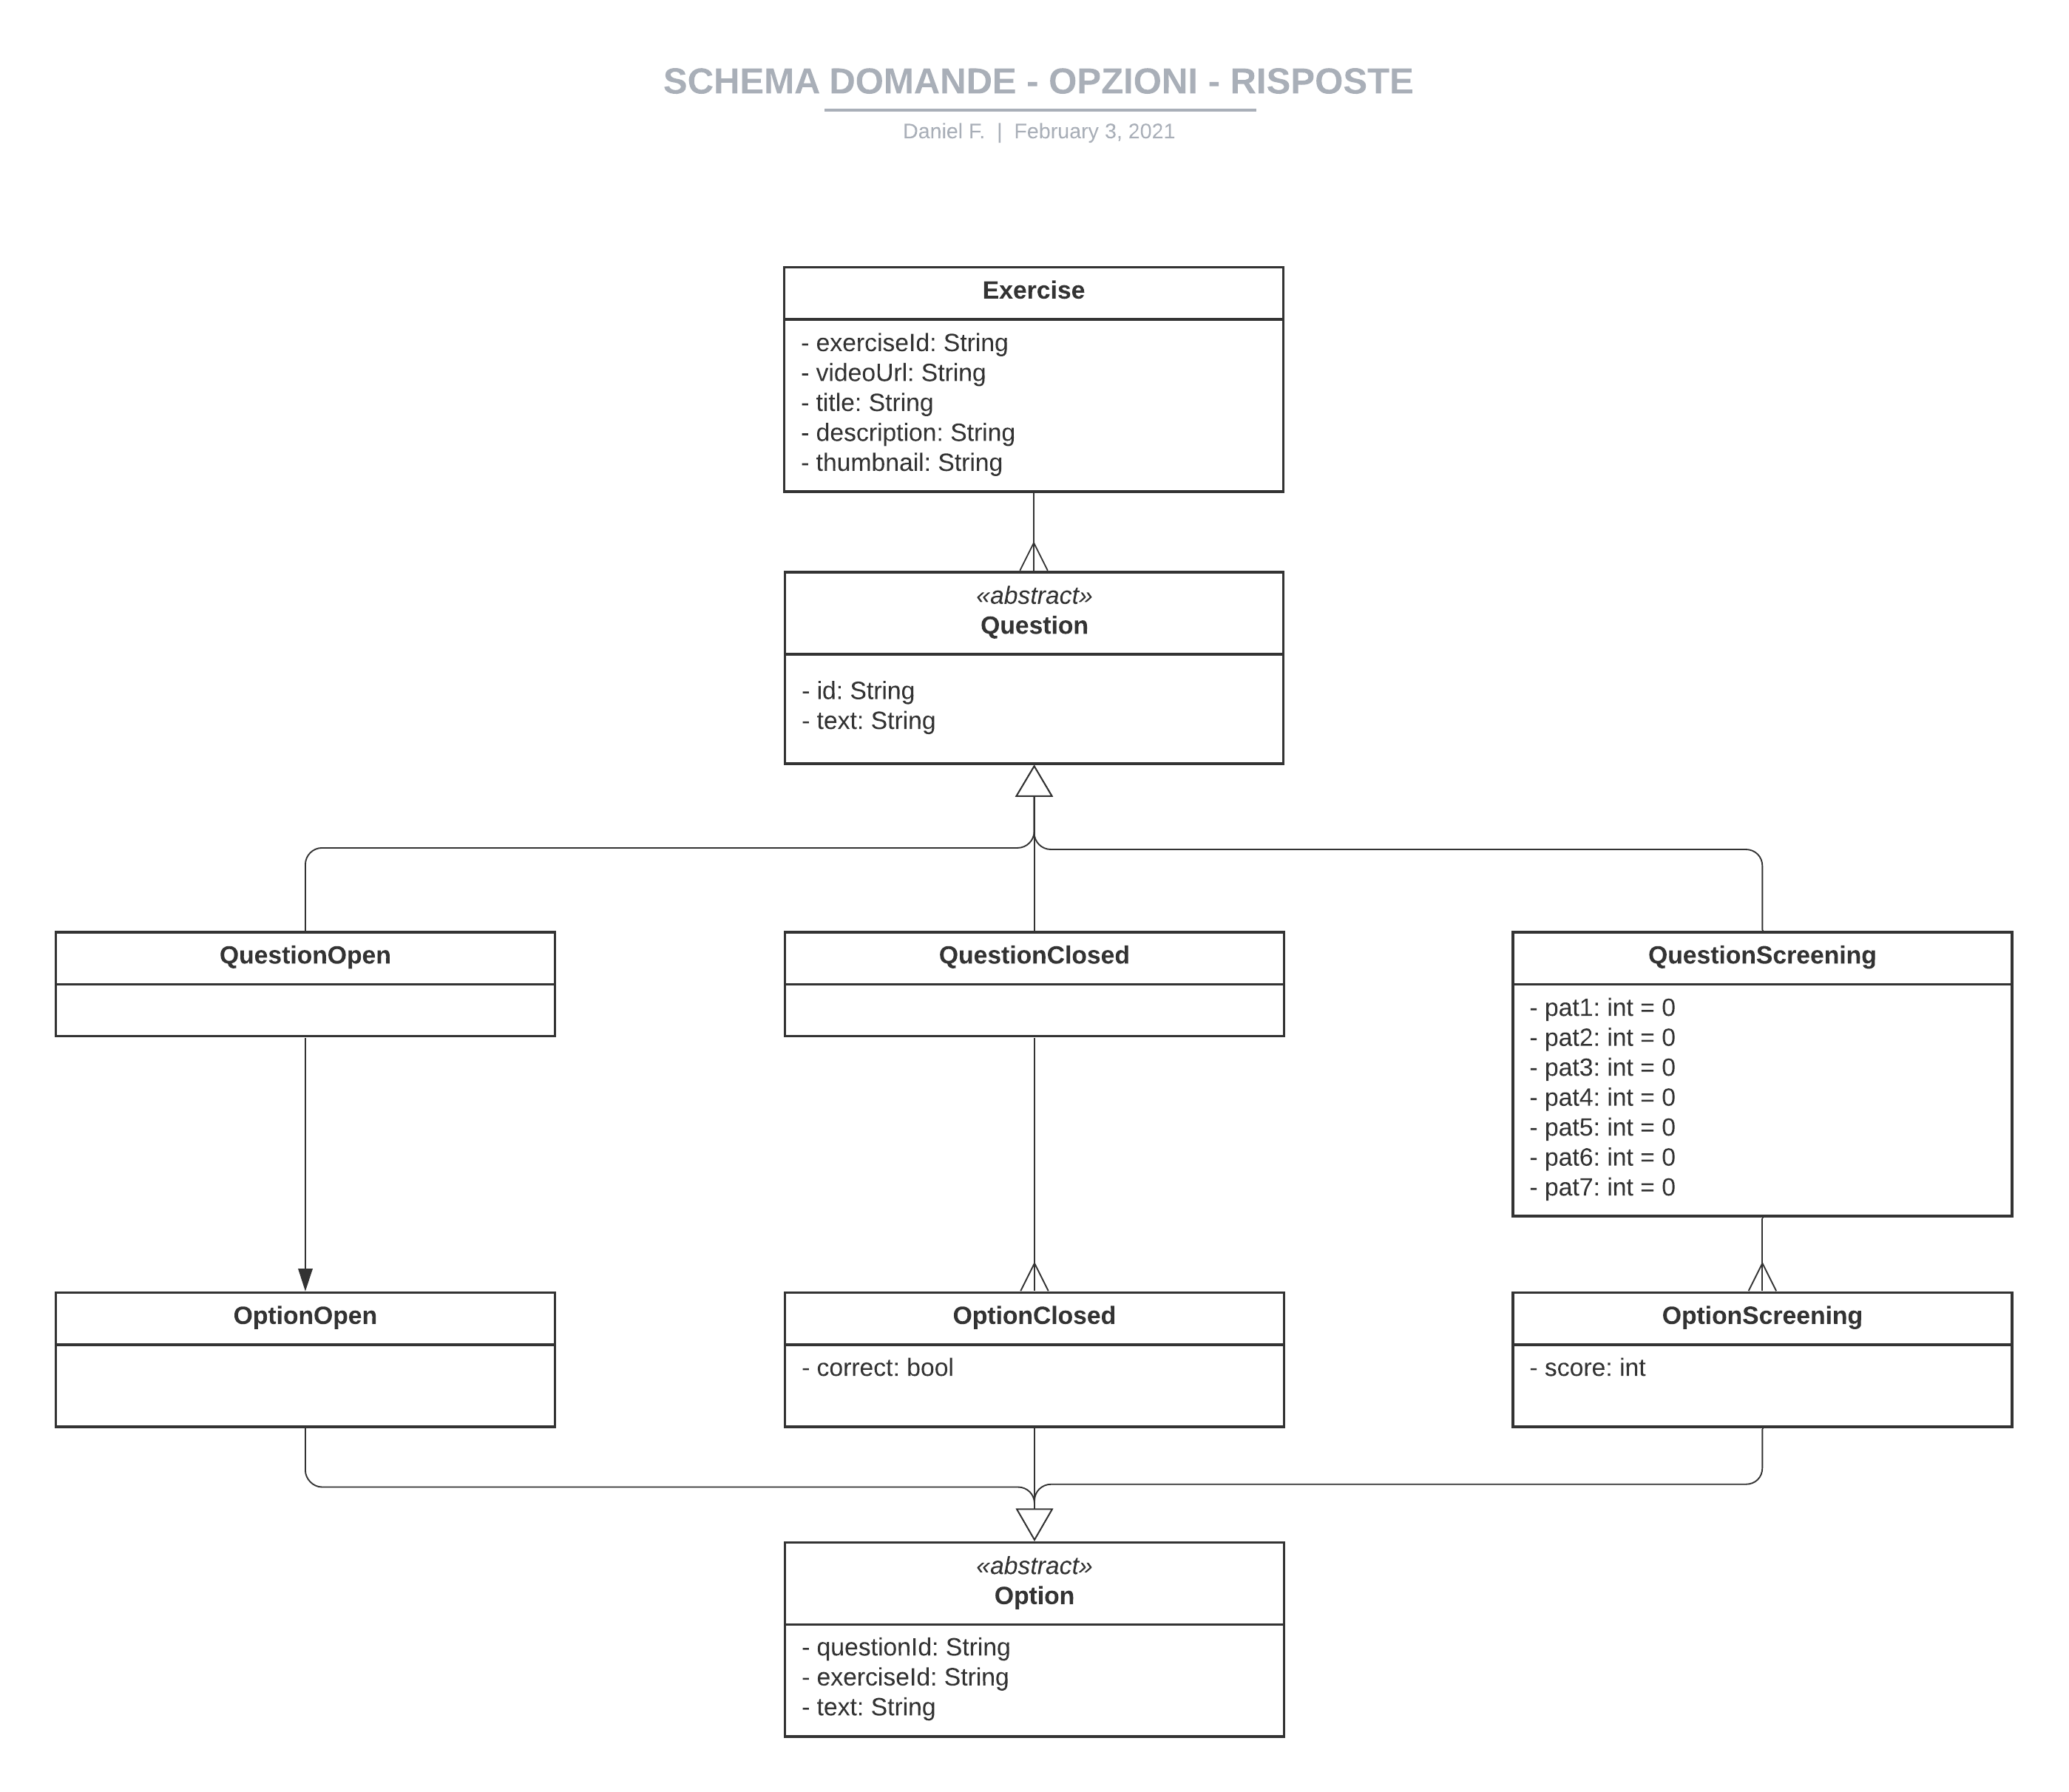
\includegraphics[width=\textwidth]{img/modello_iniziale}
\caption{Modello dati prima di Qualtrics}
\label{fig:modello_iniziale}
\end{figure}

\section{Dopo Qualtrics}
Non molto dopo i primi sviluppi è stato deciso di utilizzare \textbf{Qualtrics}\footnote{\url{www.qualtrics.com/uk/core-xm/survey-software}} come effettivo backend dell'applicazione, che non è altro che una piattaforma di creazione di sondaggi orientata alle aziende per ottenere feedback sia dai propri clienti che dai propri impiegati: l'idea era adattare questo software già pronto e che presenta già diversi tipi di domande utili al nostro scopo per poter ottenere gli input necessari dai nostri utenti e presentarli a chi di dovere. Non solo, essendo una piattaforma a sé stante, essa permette anche al gruppo di psicologia di creare i sondaggi necessari indipendentemente dallo sviluppo dell'applicazione, che si limita, tramite le API di Qualtrics, a ottenere e presentare questi sondaggi.

\subsection{Modello dati: domande}
In particolare, come possiamo vedere nel modello semplificato della Figura \ref{fig:modello_semplice_qualtrics}, il modello dati adottato da Qualtrics prevede un oggetto esterno, la \textbf{Survey} \textit{(sondaggio)}, che contiene, oltre a vari parametri di configurazione, una lista di \textbf{Questions} \textit{(domande, che sono degli oggetti anch'esse)} che possono essere di vario tipo; le domande a loro volta contengono i loro parametri di configurazione ed una lista di possibili risposte \textit{(Choices)} se a risposta chiusa.
Tra i valori interessanti contenuti nei parametri delle domande ci sono il \texttt{QuestionText}, che rappresenta la domanda vera e propria in linguaggio naturale, il \texttt{Selector} che permette di avere domande simili ma differenziate per qualche dettaglio \textit{(ad esempio possiamo avere una domanda a risposta chiusa in cui si possono selezionare più risposte piuttosto che solo una)} e il \texttt{ChoiceOrder}, che stabilisce in che ordine devono apparire le possibili risposte, contenute nell'oggetto \texttt{Choices}.
Ogni entità è inoltre opportunamente identificata, difatti le risposte non sono altro che delle coppie \texttt{<ID\_Domanda, ID\_Risposta>} oppure \texttt{<ID\_Domanda, [ID\_Risposta\_1, ..., ID\_Risposta\_n]>}, nel caso di domande a risposta chiusa, mentre nel caso di domande a risposta aperta sono del tipo \texttt{<ID\_Domanda, "Risposta">}.

\newpage

\subsection{Modello dati: blocchi}
Un aspetto particolare riguardo l'organizzazione delle domande nell'ambiente Qualtrics è quello legato ai \textbf{Blocks}, che sono degli insiemi di domande presentati separatamente. Questo permette di non sovraccaricare una schermata di domande ma di suddividerle in parti visualizzate indipendentemente.
Come si può vedere sempre nella Figura \ref{fig:modello_semplice_qualtrics}, i blocchi sono degli oggetti contenuti nell'oggetto \texttt{Survey} che dispongono di un \texttt{BlockID} e di una \texttt{Description}, una descrizione testuale utilizzata per dare un'idea del contesto delle domande presenti nel blocco. Inoltre, i blocchi contengono una lista di oggetti \texttt{BlockElements} che, seppur contente oggetti, non contiene le domande vere e proprie, ma solo gli \texttt{QuestionID} delle domande facenti parte del rispettivo blocco; è necessario quindi un incrocio dei dati nell'applicazione per far sì che le domande rispettino l'ordine dei blocchi.

È presente inoltre, sempre nell'oggetto\texttt{Survey}, un ulteriore oggetto \texttt{SurveyFlow} che contiene l'ordine di visualizzazione dei blocchi in una lista contenente i \texttt{BlockID} corrispondenti \textit{(in quanto potrebbero non essere nel giusto ordine all'interno dell'oggetto \texttt{Blocks})}.

\begin{figure}
\centering
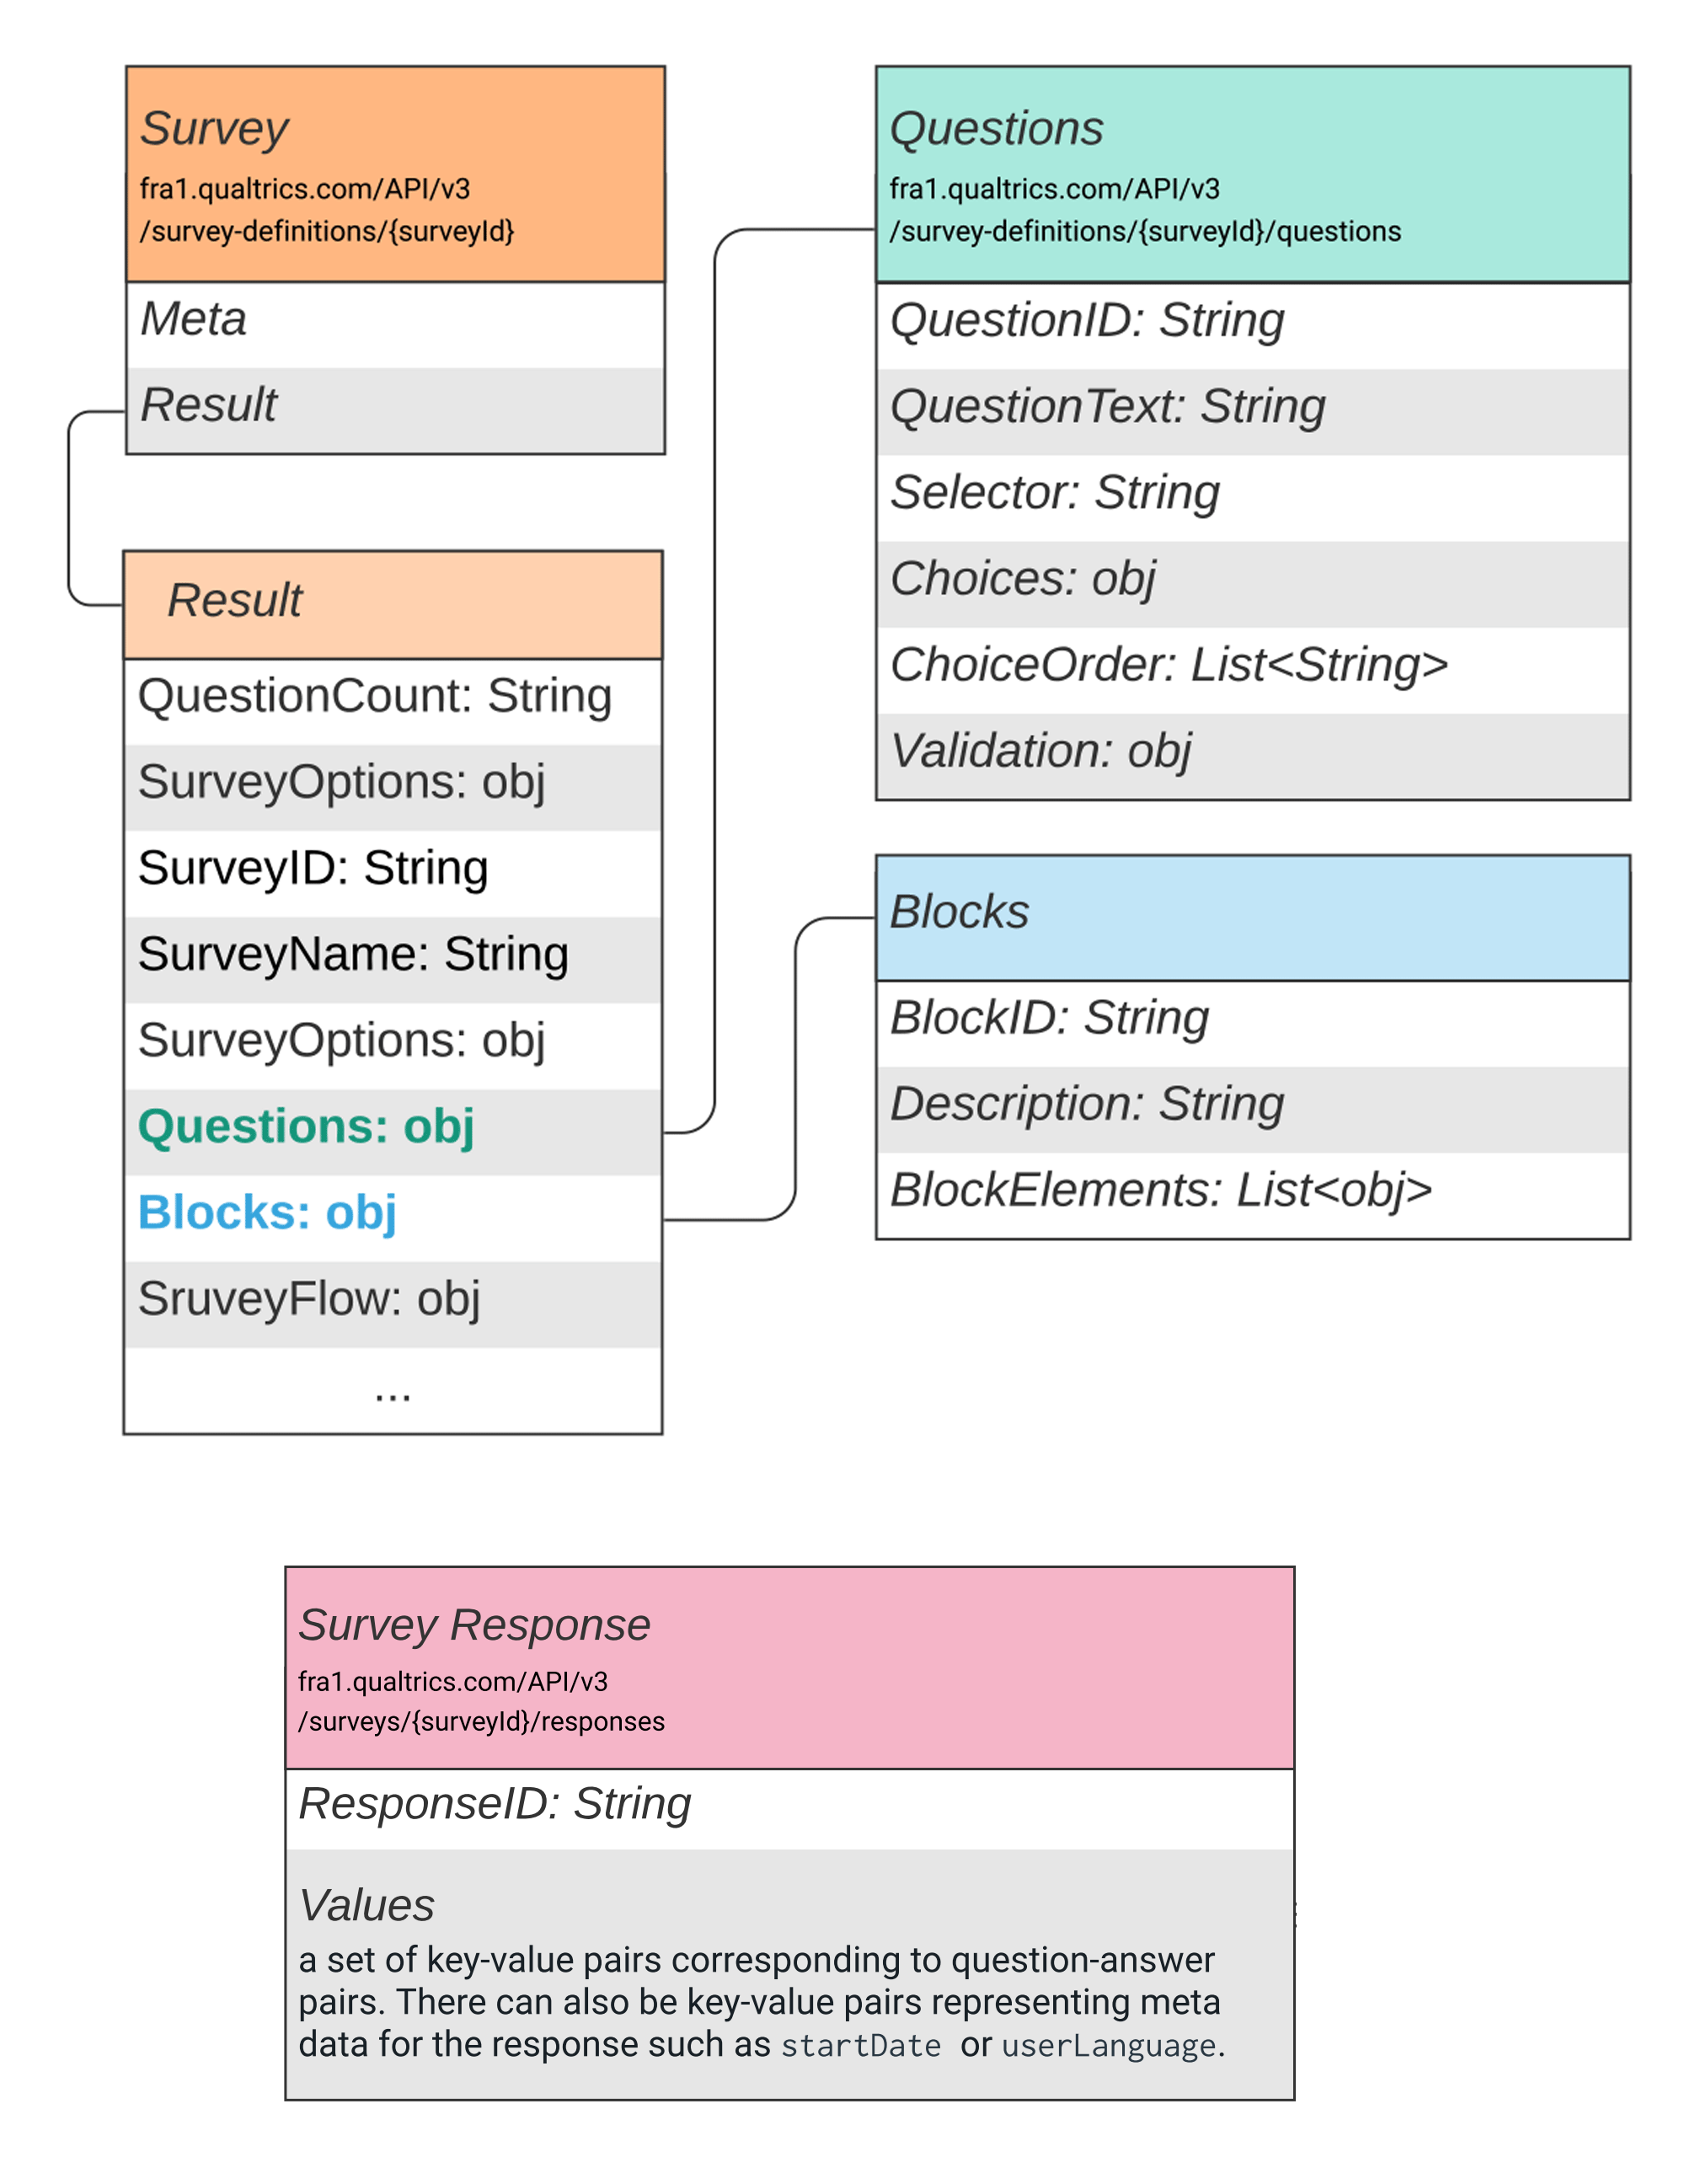
\includegraphics[width=\textwidth]{img/modello_semplice_qualtrics}
\caption{Modello dati Qualtrics semplificato}
\label{fig:modello_semplice_qualtrics}
\end{figure}

\cleardoublepage
\phantomsection
\addcontentsline{toc}{chapter}{\bibname}
\printbibliography
\end{document}	